\documentclass[conference]{IEEEtran}
\IEEEoverridecommandlockouts
\usepackage{setspace}
\usepackage{gensymb}
\singlespacing
\usepackage[cmex10]{amsmath}
\usepackage{amsthm}
\usepackage{mathrsfs}
\usepackage{txfonts}
\usepackage{stfloats}
\usepackage{bm}
\usepackage{cite}
\usepackage{cases}
\usepackage{subfig}
\usepackage{longtable}
\usepackage{multirow}
\usepackage{enumitem}
\usepackage{mathtools}
\usepackage{tikz}
\usepackage{circuitikz}
\usepackage{verbatim}
\usepackage[breaklinks=true]{hyperref}
\usepackage{tkz-euclide} % loads  TikZ and tkz-base
\usepackage{listings}
\usepackage{color}    
\usepackage{array}    
\usepackage{longtable}
\usepackage{calc}     
\usepackage{multirow} 
\usepackage{hhline}   
\usepackage{ifthen}   
\usepackage{lscape}     
\usepackage{chngcntr}
\DeclareMathOperator*{\Res}{Res}
\renewcommand\thesection{\arabic{section}}
\renewcommand\thesubsection{\thesection.\arabic{subsection}}
\renewcommand\thesubsubsection{\thesubsection.\arabic{subsubsection}}

\renewcommand\thesectiondis{\arabic{section}}
\renewcommand\thesubsectiondis{\thesectiondis.\arabic{subsection}}
\renewcommand\thesubsubsectiondis{\thesubsectiondis.\arabic{subsubsection}}
\renewcommand\thetable{\arabic{table}}
% correct bad hyphenation here
\hyphenation{op-tical net-works semi-conduc-tor}
\def\inputGnumericTable{}                                 %%

\renewcommand{\sectionautorefname}{Section}

\lstset{
%language=C,
frame=single, 
breaklines=true,
columns=fullflexible
}
%\lstset{
%language=tex,
%frame=single, 
%breaklines=true
%}

\DeclareMathOperator*{\argmax}{arg\,max}
\DeclareMathOperator*{\argmin}{arg\,min}
\begin{document}
\newtheorem{theorem}{Theorem}[section]
\newtheorem{problem}{Problem}
\newtheorem{proposition}{Proposition}[section]
\newtheorem{lemma}{Lemma}[section]
\newtheorem{corollary}[theorem]{Corollary}
\newtheorem{example}{Example}[section]
\newtheorem{definition}[problem]{Definition}
\newcommand{\BEQA}{\begin{eqnarray}}
\newcommand{\EEQA}{\end{eqnarray}}
\newcommand{\define}{\stackrel{\triangle}{=}}
\providecommand{\mbf}{\mathbf}
\providecommand{\pr}[1]{\ensuremath{\Pr\left(#1\right)}}
\providecommand{\qfunc}[1]{\ensuremath{Q\left(#1\right)}}
\providecommand{\sbrak}[1]{\ensuremath{{}\left[#1\right]}}
\providecommand{\lsbrak}[1]{\ensuremath{{}\left[#1\right.}}
\providecommand{\rsbrak}[1]{\ensuremath{{}\left.#1\right]}}
\providecommand{\brak}[1]{\ensuremath{\left(#1\right)}}
\providecommand{\lbrak}[1]{\ensuremath{\left(#1\right.}}
\providecommand{\rbrak}[1]{\ensuremath{\left.#1\right)}}
\providecommand{\cbrak}[1]{\ensuremath{\left\{#1\right\}}}
\providecommand{\lcbrak}[1]{\ensuremath{\left\{#1\right.}}
\providecommand{\rcbrak}[1]{\ensuremath{\left.#1\right\}}}
\theoremstyle{remark}
\newtheorem{rem}{Remark}
\newcommand{\sgn}{\mathop{\mathrm{sgn}}}
\providecommand{\abs}[1]{\left\vert#1\right\vert}
\providecommand{\res}[1]{\Res\displaylimits_{#1}} 
\providecommand{\norm}[1]{\left\lVert#1\right\rVert}
\providecommand{\mtx}[1]{\mathbf{#1}}
\providecommand{\mean}[1]{E\left[ #1 \right]}   
\providecommand{\fourier}{\overset{\mathcal{F}}{ \rightleftharpoons}}
\providecommand{\system}[1]{\overset{\mathcal{#1}}{ \longleftrightarrow}}
\newcommand{\solution}{\noindent \textbf{Solution: }}
\newcommand{\cosec}{\,\text{cosec}\,}
\providecommand{\dec}[2]{\ensuremath{\overset{#1}{\underset{#2}{\gtrless}}}}
\newcommand{\myvec}[1]{\ensuremath{\begin{pmatrix}#1\end{pmatrix}}}
\newcommand{\mydet}[1]{\ensuremath{\begin{vmatrix}#1\end{vmatrix}}}
\renewcommand{\vec}[1]{\boldsymbol{\mathbf{#1}}}
\def\putbox#1#2#3{\makebox[0in][l]{\makebox[#1][l]{}\raisebox{\baselineskip}[0in][0in]{\raisebox{#2}[0in][0in]{#3}}}}
     \def\rightbox#1{\makebox[0in][r]{#1}}
     \def\centbox#1{\makebox[0in]{#1}}
     \def\topbox#1{\raisebox{-\baselineskip}[0in][0in]{#1}}
     \def\midbox#1{\raisebox{-0.5\baselineskip}[0in][0in]{#1}}

\title{Unsupervised Learning for Grading Students}
\author{
    \IEEEauthorblockN{Gautam Singh and G. V. V. Sharma}
    \IEEEauthorblockA{Indian Institute of Technology, Hyderabad}
}
\maketitle

\begin{abstract}
	In this paper, we show that unsupervised learning is a superior alternative for student grading when compared to classsical Gaussian curve based methods.  This is done by applying the K-means clustering algorithm to the marks obtained by students for a particular course and qualitatively comparing it with the Gaussian approach.  \end{abstract}

\section{Introduction}
\label{sec:intro}
In recent times, especially during and after the COVID-19 pandemic, there has
been an increase in the amount of e-learning resources. Many educational
institutions have embraced online learning by using platforms such as Moodle and
have also invested in infrastructure to facilitate hybrid (both online and
in-person) classrooms. There has also been a marked increase in the number of
and amount of traffic on learning platforms such as Coursera, Udemy and edX
\cite{royEmergingTrendsApplications2017}. This boom in e-learning has led to the
collection of unique and large-scale data related to educational settings. This
has led to the emergence of the two closely related research areas of
educational data mining (EDM) and learning analytics (LA). EDM is mainly
concerned with developing methods for exploring this data, while LA is mainly
concerned with the analysis and interpretation of data about learners
\cite{romeroEducationalDataMining2020}. Both fields strive to gain actionable
insights for improving learning experiences in the form of personalized
feedback, prompt academic support, better learning strategies and holistic
evaluation methods.

In this paper, we explore the utility of unsupervised machine learning (ML)
methods for fair grading of students in a course where students performances are
skewed. We test the utility of the $K$-means clustering algorithm in assigning
letter grades as compared to grading using the Z score. We use the scores of 114
students who have taken a course in our institute. The main contributions of
this paper are as follows.

\begin{enumerate}
    \item Evaluate the utility of unsupervised learning methods as compared to
    standard methods for grading students such as using Z scores.
    \item Analyze the impact of skewed performance distributions on the fairness
    of grading.
\end{enumerate}

The remainder of this paper is structured as follows. \autoref{sec:related-work}
provides an overview of prior works related to grading of students and
assignments. \autoref{sec:methodology} describes the methods used to solve this
problem. \autoref{sec:implementation} describes the implementation details of
our approach. \autoref{sec:results} presents the results of our approach.
Finally, \autoref{sec:conclusion} concludes the paper and discusses future work.

\section{Related Work}
\label{sec:related-work}

EDM and LA encompass a wide range of fields such as education research,
educational technology, statistics, data science and artificial intelligence
\cite{WhatLearningAnalytics}. We present a brief overview of some of the works
related to grading of students using traditional methods and newer ML methods.

The most common statistic used for grading students is the \emph{Z score}
\cite{spiegelSchaumsOutlineStatistics2018}, which is defined as the number of
standard deviations a score is from the mean of the population. Apart from
scoring in standardized tests
\cite{santhanakrishnanParallelDistributedCluster2022}, the Z score is also used
to predict the financial status of companies
\cite{jagannathanPredictingBankruptcyCompanies2023} and outlier detection
\cite{yaroOutlierDetectionPerformance2024,aggarwalDetectionSpatialOutlier2019}.
However, the Z score is not a very effective measure in situations where there
are fewer students or when the performance is skewed. This leads to unfair
grading where students with similar scores end up with different grades just
because they lie on either side of a predefined boundary. Further, the Z score
can adversely impact learning experiences by intensifying academic competition
\cite{kleinAssessingUniversityStudents2014a}.

To overcome the limitations of using the Z score, researchers have appealed to
supervised and unsupervised ML methods for grading. Many studies
\cite{badalPredictiveModellingAnalytics2023,
palkhiwalaAnalysisMachineLearning2022, bujangMulticlassPredictionModel2021,
gullImprovingLearningExperience2020} have compared the performance of various
supervised and unsupervised ML algorithms for grading students in various
course, assignment and examination settings. In recent times, there has been a
marked increase in the use of unsupervised classification methods for grading
since there may not be enough labeled data for a particular course or exam
collected to sufficiently train a supervised model. In particular, clustering
methods have become a key technology for EDM and LA
\cite{zhangBriefAnalysisKey2018}. A particularly popular clustering method used
in many studies is the $K$-means clustering algorithm
\cite{macqueenMethodsClassificationAnalysis1967}. The authors of
\cite{bucosStudentClusterAnalysis2020} were able to use the $K$-means algorithm
to identify students at risk of failing to complete coursework by collecting
data pertaining to a single course offered over many years. In
\cite{wangAlgorithmStudentGrade2022}, the $K$-means algorithm was used to promptly
identify and guide students at the edge of the grading classification. Variants
of the original $K$-means algorithm have also been used for grading students.
The $K$-means++ algorithm was used by the authors of
\cite{jimenez-maciasStudentClusteringKMeans2024} to enhance the quality of
assignments given to students. The authors of
\cite{bhartiCentroidBasedClustering2024} evaluated the utility of the
$K$-medians algorithm along with the $K$-means algorithm for determining the
rankings of schools in a common examination. However, the aforementioned studies
do not evaluate the performance of clustering algorithms in scenarios where the
performance of students is skewed. We aim to fill this gap by comparing the
utility of $K$-means clustering in assigning grades in such a scenario.

\section{Methodology}
\label{sec:methodology}

\subsection{Z Score}
For a given dataset $\cbrak{X_1, X_2, \ldots, X_N}$ of size $N$, we can compute
the population mean and population variance using the following equations.
\begin{align}
    \mu = \mean{X} &= \frac{1}{N}\sum_{i=1}^N X_i \\
    \sigma^2 = \mean{\brak{X-\mu}^2} &= \frac{1}{N}\sum_{i=1}^N\brak{X_i-\mu}^2
    \label{eq:pop-param}
\end{align}

Using the central limit theorem \cite{spiegelSchaumsOutlineStatistics2018}, we
assume that the scores $X \sim N\brak{\mu,\sigma^2}$. Thus, the $Z$-score of $X$
is given by
\begin{equation}
    Z = \frac{X-\mu}{\sigma}.
\end{equation}

The letter grades are assigned as per \autoref{tab:grade-scheme}.
\begin{table}[!ht]
    \centering
    %%%%%%%%%%%%%%%%%%%%%%%%%%%%%%%%%%%%%%%%%%%%%%%%%%%%%%%%%%%%%%%%%%%%%%
%%                                                                  %%
%%  This is the header of a LaTeX2e file exported from Gnumeric.    %%
%%                                                                  %%
%%  This file can be compiled as it stands or included in another   %%
%%  LaTeX document. The table is based on the longtable package so  %%
%%  the longtable options (headers, footers...) can be set in the   %%
%%  preamble section below (see PRAMBLE).                           %%
%%                                                                  %%
%%  To include the file in another, the following two lines must be %%
%%  in the including file:                                          %%
%%        \def\inputGnumericTable{}                                 %%
%%  at the beginning of the file and:                               %%
%%        \input{name-of-this-file.tex}                             %%
%%  where the table is to be placed. Note also that the including   %%
%%  file must use the following packages for the table to be        %%
%%  rendered correctly:                                             %%
%%    \usepackage[latin1]{inputenc}                                 %%
%%    \usepackage{color}                                            %%
%%    \usepackage{array}                                            %%
%%    \usepackage{longtable}                                        %%
%%    \usepackage{calc}                                             %%
%%    \usepackage{multirow}                                         %%
%%    \usepackage{hhline}                                           %%
%%    \usepackage{ifthen}                                           %%
%%  optionally (for landscape tables embedded in another document): %%
%%    \usepackage{lscape}                                           %%
%%                                                                  %%
%%%%%%%%%%%%%%%%%%%%%%%%%%%%%%%%%%%%%%%%%%%%%%%%%%%%%%%%%%%%%%%%%%%%%%



%%  This section checks if we are begin input into another file or  %%
%%  the file will be compiled alone. First use a macro taken from   %%
%%  the TeXbook ex 7.7 (suggestion of Han-Wen Nienhuys).            %%
\def\ifundefined#1{\expandafter\ifx\csname#1\endcsname\relax}


%%  Check for the \def token for inputed files. If it is not        %%
%%  defined, the file will be processed as a standalone and the     %%
%%  preamble will be used.                                          %%
\ifundefined{inputGnumericTable}

%%  We must be able to close or not the document at the end.        %%
	\def\gnumericTableEnd{\end{document}}


%%%%%%%%%%%%%%%%%%%%%%%%%%%%%%%%%%%%%%%%%%%%%%%%%%%%%%%%%%%%%%%%%%%%%%
%%                                                                  %%
%%  This is the PREAMBLE. Change these values to get the right      %%
%%  paper size and other niceties.                                  %%
%%                                                                  %%
%%%%%%%%%%%%%%%%%%%%%%%%%%%%%%%%%%%%%%%%%%%%%%%%%%%%%%%%%%%%%%%%%%%%%%

	\documentclass[12pt%
			  %,landscape%
                    ]{report}
       \usepackage[latin1]{inputenc}
       \usepackage{fullpage}
       \usepackage{color}
       \usepackage{array}
       \usepackage{longtable}
       \usepackage{calc}
       \usepackage{multirow}
       \usepackage{hhline}
       \usepackage{ifthen}

	\begin{document}


%%  End of the preamble for the standalone. The next section is for %%
%%  documents which are included into other LaTeX2e files.          %%
\else

%%  We are not a stand alone document. For a regular table, we will %%
%%  have no preamble and only define the closing to mean nothing.   %%
    \def\gnumericTableEnd{}

%%  If we want landscape mode in an embedded document, comment out  %%
%%  the line above and uncomment the two below. The table will      %%
%%  begin on a new page and run in landscape mode.                  %%
%       \def\gnumericTableEnd{\end{landscape}}
%       \begin{landscape}


%%  End of the else clause for this file being \input.              %%
\fi

%%%%%%%%%%%%%%%%%%%%%%%%%%%%%%%%%%%%%%%%%%%%%%%%%%%%%%%%%%%%%%%%%%%%%%
%%                                                                  %%
%%  The rest is the gnumeric table, except for the closing          %%
%%  statement. Changes below will alter the table's appearance.     %%
%%                                                                  %%
%%%%%%%%%%%%%%%%%%%%%%%%%%%%%%%%%%%%%%%%%%%%%%%%%%%%%%%%%%%%%%%%%%%%%%

\providecommand{\gnumericmathit}[1]{#1} 
%%  Uncomment the next line if you would like your numbers to be in %%
%%  italics if they are italizised in the gnumeric table.           %%
%\renewcommand{\gnumericmathit}[1]{\mathit{#1}}
\providecommand{\gnumericPB}[1]%
{\let\gnumericTemp=\\#1\let\\=\gnumericTemp\hspace{0pt}}
 \ifundefined{gnumericTableWidthDefined}
        \newlength{\gnumericTableWidth}
        \newlength{\gnumericTableWidthComplete}
        \newlength{\gnumericMultiRowLength}
        \global\def\gnumericTableWidthDefined{}
 \fi
%% The following setting protects this code from babel shorthands.  %%
 \ifthenelse{\isundefined{\languageshorthands}}{}{\languageshorthands{english}}
%%  The default table format retains the relative column widths of  %%
%%  gnumeric. They can easily be changed to c, r or l. In that case %%
%%  you may want to comment out the next line and uncomment the one %%
%%  thereafter                                                      %%
\providecommand\gnumbox{\makebox[0pt]}
%%\providecommand\gnumbox[1][]{\makebox}

%% to adjust positions in multirow situations                       %%
\setlength{\bigstrutjot}{\jot}
\setlength{\extrarowheight}{\doublerulesep}

%%  The \setlongtables command keeps column widths the same across  %%
%%  pages. Simply comment out next line for varying column widths.  %%
\setlongtables

\setlength\gnumericTableWidth{%
	53pt+%
	53pt+%
0pt}
\def\gumericNumCols{2}
\setlength\gnumericTableWidthComplete{\gnumericTableWidth+%
         \tabcolsep*\gumericNumCols*2+\arrayrulewidth*\gumericNumCols}
\ifthenelse{\lengthtest{\gnumericTableWidthComplete > \linewidth}}%
         {\def\gnumericScale{\ratio{\linewidth-%
                        \tabcolsep*\gumericNumCols*2-%
                        \arrayrulewidth*\gumericNumCols}%
{\gnumericTableWidth}}}%
{\def\gnumericScale{1}}

%%%%%%%%%%%%%%%%%%%%%%%%%%%%%%%%%%%%%%%%%%%%%%%%%%%%%%%%%%%%%%%%%%%%%%
%%                                                                  %%
%% The following are the widths of the various columns. We are      %%
%% defining them here because then they are easier to change.       %%
%% Depending on the cell formats we may use them more than once.    %%
%%                                                                  %%
%%%%%%%%%%%%%%%%%%%%%%%%%%%%%%%%%%%%%%%%%%%%%%%%%%%%%%%%%%%%%%%%%%%%%%

\ifthenelse{\isundefined{\gnumericColA}}{\newlength{\gnumericColA}}{}\settowidth{\gnumericColA}{\begin{tabular}{@{}p{53pt*\gnumericScale}@{}}x\end{tabular}}
\ifthenelse{\isundefined{\gnumericColB}}{\newlength{\gnumericColB}}{}\settowidth{\gnumericColB}{\begin{tabular}{@{}p{53pt*\gnumericScale}@{}}x\end{tabular}}

\begin{tabular}[c]{%
	b{\gnumericColA}%
	b{\gnumericColB}%
	}

%%%%%%%%%%%%%%%%%%%%%%%%%%%%%%%%%%%%%%%%%%%%%%%%%%%%%%%%%%%%%%%%%%%%%%
%%  The longtable options. (Caption, headers... see Goosens, p.124) %%
%	\caption{The Table Caption.}             \\	%
% \hline	% Across the top of the table.
%%  The rest of these options are table rows which are placed on    %%
%%  the first, last or every page. Use \multicolumn if you want.    %%

%%  Header for the first page.                                      %%
%	\multicolumn{2}{c}{The First Header} \\ \hline 
%	\multicolumn{1}{c}{colTag}	%Column 1
%	&\multicolumn{1}{c}{colTag}	\\ \hline %Last column
%	\endfirsthead

%%  The running header definition.                                  %%
%	\hline
%	\multicolumn{2}{l}{\ldots\small\slshape continued} \\ \hline
%	\multicolumn{1}{c}{colTag}	%Column 1
%	&\multicolumn{1}{c}{colTag}	\\ \hline %Last column
%	\endhead

%%  The running footer definition.                                  %%
%	\hline
%	\multicolumn{2}{r}{\small\slshape continued\ldots} \\
%	\endfoot

%%  The ending footer definition.                                   %%
%	\multicolumn{2}{c}{That's all folks} \\ \hline 
%	\endlastfoot
%%%%%%%%%%%%%%%%%%%%%%%%%%%%%%%%%%%%%%%%%%%%%%%%%%%%%%%%%%%%%%%%%%%%%%

\hhline{|-|-}
	 \multicolumn{1}{|p{\gnumericColA}|}%
	{\gnumericPB{\raggedright}\gnumbox[l]{\textbf{Interval}}}
	&\multicolumn{1}{p{\gnumericColB}|}%
	{\gnumericPB{\raggedright}\gnumbox[l]{\textbf{Grade}}}
\\
\hhline{|--|}
	 \multicolumn{1}{|p{\gnumericColA}|}%
	{\gnumericPB{\raggedright}\gnumbox[l]{($-\infty$, -3]}}
	&\multicolumn{1}{p{\gnumericColB}|}%
	{\gnumericPB{\raggedright}\gnumbox[l]{F}}
\\
\hhline{|--|}
	 \multicolumn{1}{|p{\gnumericColA}|}%
	{\gnumericPB{\raggedright}\gnumbox[l]{(-3, -2]}}
	&\multicolumn{1}{p{\gnumericColB}|}%
	{\gnumericPB{\raggedright}\gnumbox[l]{D}}
\\
\hhline{|--|}
	 \multicolumn{1}{|p{\gnumericColA}|}%
	{\gnumericPB{\raggedright}\gnumbox[l]{(-2, 1]}}
	&\multicolumn{1}{p{\gnumericColB}|}%
	{\gnumericPB{\raggedright}\gnumbox[l]{C}}
\\
\hhline{|--|}
	 \multicolumn{1}{|p{\gnumericColA}|}%
	{\gnumericPB{\raggedright}\gnumbox[l]{(-1, 0]}}
	&\multicolumn{1}{p{\gnumericColB}|}%
	{\gnumericPB{\raggedright}\gnumbox[l]{B-}}
\\
\hhline{|--|}
	 \multicolumn{1}{|p{\gnumericColA}|}%
	{\gnumericPB{\raggedright}\gnumbox[l]{(0, 1]}}
	&\multicolumn{1}{p{\gnumericColB}|}%
	{\gnumericPB{\raggedright}\gnumbox[l]{B}}
\\
\hhline{|--|}
	 \multicolumn{1}{|p{\gnumericColA}|}%
	{\gnumericPB{\raggedright}\gnumbox[l]{(1, 2]}}
	&\multicolumn{1}{p{\gnumericColB}|}%
	{\gnumericPB{\raggedright}\gnumbox[l]{A-}}
\\
\hhline{|--|}
	 \multicolumn{1}{|p{\gnumericColA}|}%
	{\gnumericPB{\raggedright}\gnumbox[l]{(2, 3]}}
	&\multicolumn{1}{p{\gnumericColB}|}%
	{\gnumericPB{\raggedright}\gnumbox[l]{A}}
\\
\hhline{|--|}
	 \multicolumn{1}{|p{\gnumericColA}|}%
	{\gnumericPB{\raggedright}\gnumbox[l]{(3,$\infty$)}}
	&\multicolumn{1}{p{\gnumericColB}|}%
	{\gnumericPB{\raggedright}\gnumbox[l]{A+}}
\\
\hhline{|-|-|}
\end{tabular}

\ifthenelse{\isundefined{\languageshorthands}}{}{\languageshorthands{\languagename}}
\gnumericTableEnd

    \caption{Grading Scheme.}
    \label{tab:grade-scheme}
\end{table}

\subsection{K-Means Clustering}
$K$-Means clustering \cite{macqueenMethodsClassificationAnalysis1967} is an
unsupervised classification model, which attempts to cluster unlabeled data in
order to gain more structure from it. 

To find the optimum means for a fixed number of letter grades as per
\autoref{tab:grade-scheme}, we frame the problem of assigning letter grades as
an optimization problem. For a set of data points $\cbrak{\vec{X}_i}_{i=1}^N$
and means $\cbrak{\vec{\mu}_i}_{i=1}^K$, we define for $1 \le n \le N,\ 1 \le k
\le K$,
\begin{equation}
    r_{nk} \triangleq
    \begin{cases}
        1 & \argmin_{j}\norm{\vec{X}_n-\vec{\mu}_j} = k \\
        0 & \textrm{otherwise}
    \end{cases}
    \label{eq:rnk-def}
\end{equation}
Thus, we need to find points $\vec{\mu}_k$ minimizing the cost function
\begin{equation}
    J \triangleq \sum_{n=1}^N\sum_{k=1}^Kr_{nk}\norm{\vec{X}_n-\vec{\mu}_k}^2
    \label{eq:cost}
\end{equation}
Clearly, \eqref{eq:cost} is a quadratic function of $\vec{\mu}_k$.
Differentiating with respect to $\vec{\mu}_k$ and setting the derivative to
zero, we get
\begin{align}
    \sum_{n=1}^N2\vec{\mu}_kr_{nk}\brak{\vec{x}_n-\vec{\mu}_k} = 0 \\
    \implies \vec{\mu_k} = \frac{\sum_{n=1}^Nr_{nk}\vec{x}_n}{\sum_{n=1}^Nr_{nk}} = \frac{\vec{Xr}_k}{\vec{1}^\top\vec{r}_k}
    \label{eq:M-step}
\end{align}
where
\begin{align}
    \vec{X} &\triangleq \myvec{\vec{X}_1&\vec{X}_2&\ldots&\vec{X}_n} \\
    \vec{r}_k &\triangleq \myvec{r_{1k}&r_{2k}&\ldots&r_{nk}}^\top \\
    \vec{1} &\triangleq \myvec{1&1&\ldots&1}^\top
    \label{eq:M-defs}
\end{align}
From \eqref{eq:M-step}, we see that the optimum is attained when $\vec{\mu}_k$
is set to the expectation of the $\vec{X}_n$ with respect to $r_{nk}$.

Thus, the $K$-means algorithm is an \emph{expectation maximization} (EM)
algorithm where each iteration consists of two steps until convergence.
\begin{enumerate}
    \item \emph{Expectation Step} (E Step): For $1 \le k \le K$, calculate the
    expected means using \eqref{eq:E-step}.
    \begin{equation}
        \tilde{\vec{\mu}_k} \triangleq \frac{\sum_{n=1}^Nr_{nk}\vec{X}_n}{\sum_{n=1}^Nr_{nk}}
        \label{eq:E-step}
    \end{equation}
    \item \emph{Maximization Step} (M Step): Set $\vec{\mu}_k \leftarrow
    \tilde{\vec{\mu}_k}$ for $1 \le k \le K$.
\end{enumerate}

\section{Implementation}
\label{sec:implementation}

A sample of ten rows of the dataset used for grading is shown in
\autoref{tab:sample-data}. The dataset contains the scores of 114 students who
have taken a course in our institute, where the maximum score is 100.
\begin{table}[!ht]
    \centering
    \begin{tabular}{|c|c|}
        \hline
        \textbf{S.No.} & \textbf{Marks} \\
        \hline
        1 & 46.8 \\
        \hline
        2 & 76 \\
        \hline
        3 & 11 \\
        \hline
        4 & 53 \\
        \hline
        5 & 31.5 \\
        \hline
        6 & 34.5 \\
        \hline
        7 & 55 \\
        \hline
        8 & 51.6 \\
        \hline
        9 & 23.2 \\
        \hline
        10 & 0 \\
        \hline
    \end{tabular}
    \caption{Sample of the dataset used for grading.}
    \label{tab:sample-data}
\end{table}

We implemented the Z score algorithm as well as the EM algorithm for the
$K$-means clustering algorithm in Python using the \texttt{numpy} and
\texttt{pandas} libraries. The raw data is collected in the \texttt{marks.xlsx}
file. The source codes and dataset are openly available on
\href{https://github.com/gadepall/grading}{GitHub}.

The Python code \texttt{codes/grades\_norm.py} takes the given input population
dataset \texttt{marks.xlsx} and assigns grades appropriately. The grades are
output to \texttt{grades\_norm.xlsx}. A similar task is performed by the
\texttt{codes/grades\_kmeans.py} code, which uses the $K$-means algorithm to
assign grades and outputs the results to \texttt{grades\_kmeans.xlsx}.

\section{Results}
\label{sec:results}
The grade distribution using each method is shown in \autoref {fig:gauss-dist}
and \autoref{fig:kmeans-dist}. In particular, the grades assigned for the sample
data presented in \autoref{tab:sample-data} is shown in
\autoref{tab:grade-assignment}.
\begin{figure}[!ht]
    \centering
    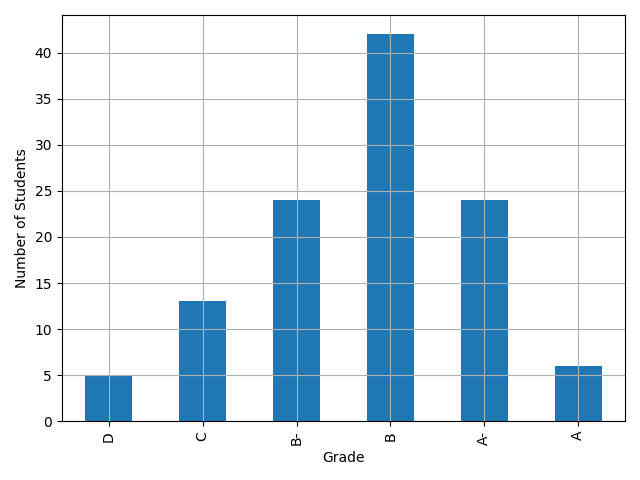
\includegraphics[width=\columnwidth]{figs/grades_gauss.png}
    \caption{Grade distribution using Z scores.}
    \label{fig:gauss-dist}
\end{figure}
\begin{figure}[!ht]
    \centering
    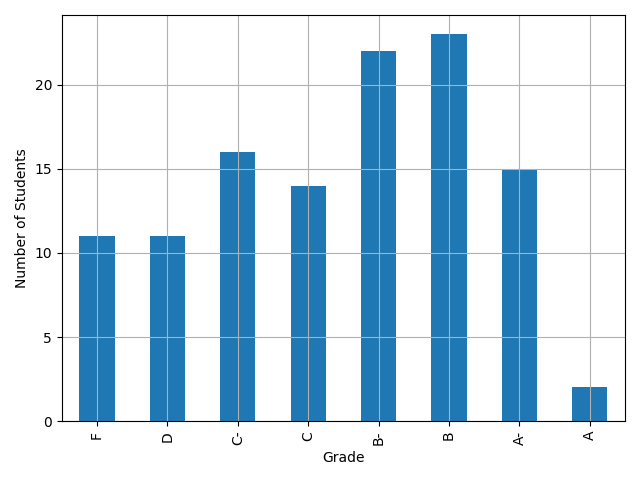
\includegraphics[width=\columnwidth]{figs/grades_kmeans.png}
    \caption{Grade distribution using the $K$-means algorithm.}
    \label{fig:kmeans-dist}
\end{figure}
\begin{table}[!h]
    \centering
    \begin{tabular}{|c|c|c|c|}
        \hline
        \textbf{S.No.} & \textbf{Marks} & \textbf{Grade (Z Score)} & \textbf{Grade (K Means)} \\
        \hline
        1 & 46.8 & B & B- \\
        \hline
        2 & 76 & A & A- \\
        \hline
        3 & 11 & C & D \\
        \hline
        4 & 53 & B & B- \\
        \hline
        5 & 31.5 & B- & C- \\
        \hline
        6 & 34.5 & B- & C- \\
        \hline
        7 & 55 & B & B \\
        \hline
        8 & 51.6 & B & B- \\
        \hline
        9 & 23.2 & B- & D \\
        \hline
        10 & 0 & D & F \\
        \hline
    \end{tabular}
    \caption{Grade assignment for a sample of students using both methods.}
    \label{tab:grade-assignment}
\end{table}

Based on the results, we can make the following observations:
\begin{enumerate}
    \item Using the Gaussian distribution is quite unfair, since there could be
    students with quite similar marks but with a difference in grade, just
    because they lie on either side of a predefined boundary.
    \item The $K$-means algorithm allows for better decision boundaries,
    depending on how skewed the performance of the students is, accordingly to
    the difficulty of the course.
    \item Unlike the Gaussian distribution, the $K$-means algorithm can be used
    for a fairer assignment of the grades, no matter how skewed the performance
    of students in a course is.
\end{enumerate}

\section{Conclusion and Future Work}
\label{sec:conclusion}

In this paper, we analyzed the utility of unsupervised learning methods for
grading students in a course where the performance of students is skewed. We
compared the performance of the $K$-means algorithm with using Z scores in
assigning grades to students. Our results indicate that the $K$-means algorithm
is more effective in handling skewed distributions and providing fairer grade
assignments. A possible future extension can be to explore the utility of other
unsupervised learning algorithms with datasets containing more features
collected over a period of time. Another possible extension could be to
integrate these methods with existing content management systems to provide
continuous and personalized feedback to students.

\bibliographystyle{IEEEtran}
\bibliography{references}

\end{document}
